\documentclass[12pt]{article}

\usepackage{amsmath, mathtools}
\usepackage{amsfonts}
\usepackage{amssymb}
\usepackage{graphicx}
\usepackage{colortbl}
\usepackage{xr}
\usepackage{hyperref}
\usepackage{longtable}
\usepackage{xfrac}
\usepackage{tabularx}
\usepackage{float}
\usepackage{siunitx}
\usepackage{soul}
\usepackage{booktabs}
\usepackage{caption}
\usepackage{pdflscape}
\usepackage{afterpage}
\usepackage{enumerate}


\usepackage[round]{natbib}

%\usepackage{refcheck}

\hypersetup{
    %bookmarks=true,         % show bookmarks bar?
      colorlinks=true,       % false: boxed links; true: colored links
    linkcolor=red,          % color of internal links (change box color with linkbordercolor)
    citecolor=green,        % color of links to bibliography
    filecolor=magenta,      % color of file links
    urlcolor=cyan           % color of external links
}

%% Comments

\usepackage{color}

\newif\ifcomments\commentstrue %displays comments
%\newif\ifcomments\commentsfalse %so that comments do not display

\ifcomments
\newcommand{\authornote}[3]{\textcolor{#1}{[#3 ---#2]}}
\newcommand{\todo}[1]{\textcolor{red}{[TODO: #1]}}
\else
\newcommand{\authornote}[3]{}
\newcommand{\todo}[1]{}
\fi

\newcommand{\wss}[1]{\authornote{blue}{SS}{#1}} 
\newcommand{\plt}[1]{\authornote{magenta}{TPLT}{#1}} %For explanation of the template
\newcommand{\an}[1]{\authornote{cyan}{Author}{#1}}

%% Common Parts

\newcommand{\progname}{ProgName} % PUT YOUR PROGRAM NAME HERE
\newcommand{\authname}{Team \#, Team Name
\\ Student 1 name
\\ Student 2 name
\\ Student 3 name
\\ Student 4 name} % AUTHOR NAMES                  

\usepackage{hyperref}
    \hypersetup{colorlinks=true, linkcolor=blue, citecolor=blue, filecolor=blue,
                urlcolor=blue, unicode=false}
    \urlstyle{same}
                                


% For easy change of table widths
\newcommand{\colZwidth}{1.0\textwidth}
\newcommand{\colAwidth}{0.13\textwidth}
\newcommand{\colBwidth}{0.82\textwidth}
\newcommand{\colCwidth}{0.1\textwidth}
\newcommand{\colDwidth}{0.05\textwidth}
\newcommand{\colEwidth}{0.8\textwidth}
\newcommand{\colFwidth}{0.17\textwidth}
\newcommand{\colGwidth}{0.5\textwidth}
\newcommand{\colHwidth}{0.28\textwidth}
\newcommand{\tableVspace}{5mm}

% Used so that cross-references have a meaningful prefix
\newcounter{defnum} %Definition Number
\newcommand{\dthedefnum}{GD\thedefnum}
\newcommand{\dref}[1]{GD\ref{#1}}
\newcounter{datadefnum} %Datadefinition Number
\newcommand{\ddthedatadefnum}{DD\thedatadefnum}
\newcommand{\ddref}[1]{DD\ref{#1}}
\newcounter{theorynum} %Theory Number
\newcommand{\tthetheorynum}{T\thetheorynum}
\newcommand{\tref}[1]{T\ref{#1}}
\newcounter{tablenum} %Table Number
\newcommand{\tbthetablenum}{T\thetablenum}
\newcommand{\tbref}[1]{TB\ref{#1}}
\newcounter{assumpnum} %Assumption Number
\newcommand{\atheassumpnum}{P\theassumpnum}
\newcommand{\aref}[1]{A\ref{#1}}
\newcounter{goalnum} %Goal Number
\newcommand{\gthegoalnum}{P\thegoalnum}
\newcommand{\gsref}[1]{GS\ref{#1}}
\newcounter{instnum} %Instance Number
\newcommand{\itheinstnum}{IM\theinstnum}
\newcommand{\iref}[1]{IM\ref{#1}}
\newcounter{reqnum} %Requirement Number
\newcommand{\rthereqnum}{P\thereqnum}
\newcommand{\rref}[1]{R\ref{#1}}
\newcounter{nfrnum} %NFR Number
\newcommand{\rthenfrnum}{NFR\thenfrnum}
\newcommand{\nfrref}[1]{NFR\ref{#1}}
\newcounter{lcnum} %Likely change number
\newcommand{\lthelcnum}{LC\thelcnum}
\newcommand{\lcref}[1]{LC\ref{#1}}
\newcommand{\ReqColA}{0.13\textwidth}
\newcommand{\ReqColB}{0.82\textwidth}

\usepackage{fullpage}

\graphicspath{{Figures/}}

\newcommand{\deftheory}[9][Not Applicable]
{
\newpage
\noindent \rule{\textwidth}{0.5mm}

\paragraph{RefName: } \textbf{#2} \phantomsection 
\label{#2}

\paragraph{Label:} #3

\noindent \rule{\textwidth}{0.5mm}

\paragraph{Equation:}

#4

\paragraph{Description:}

#5

\paragraph{Notes:}

#6

\paragraph{Source:}

#7

\paragraph{Ref.\ By:}

#8

\paragraph{Preconditions for \hyperref[#2]{#2}:}
\label{#2_precond}

#9

\paragraph{Derivation for \hyperref[#2]{#2}:}
\label{#2_deriv}

#1

\noindent \rule{\textwidth}{0.5mm}

}

\begin{document}

\title{Software Requirements Specification for \progname: \bf Formula Electric Vehicle Control System} 
\author{\authname}
\date{\today}
	
\maketitle

~\newpage

\pagenumbering{arabic}

\tableofcontents

~\newpage

\section*{Revision History}

\begin{tabularx}{\textwidth}{p{3cm}p{2cm}X}
\toprule {\bf Date} & {\bf Version} & {\bf Notes}\\
\midrule
Oct 5th, 2022 & 1.0 & Initial Revision\\
\bottomrule
\end{tabularx}

~\newpage

\section{Project Drivers}

\subsection{The Purpose of the Project}

The purpose of this project will be to design, simulate, implement, and test a fully functioning vehicle control system 
for a quarter-scale Formula 1 style electric vehicle.
Currently, the McMaster Formula Electric team is in the process of preparing their vehicle for the FSAE competition taking 
place in Michigan next summer. During the 2020 Fall - 2021 Winter term of the school year, the team went through a full redesign of the
electrical and embedded system architecture. The new architecture included a switch from Atmel to STM32F7 microprocessors, enabling the team to develop, test, and 
integrate in-house vehicle software for their ECUs. This change allows us to implement our own custom vehicle controls software.

\subsection{Scope}

The control system will be responsible for managing the following vehicle subsystems: battery management, vehicle mode selection, tractive motor, and vehicle dynamics.

\subsection{Typical Operations Overview}

A student on the McMaster Formula Electric team, who is familiar with the basics of Matlab, can push the finished
vehicle controls model to the respective ECU's that exist in the vehicle. In terms of adjust things like sensitivity, a 
student can enter the model and change values that are presented to them. This can adjust things like brake \& accelerator 
sensitivity, how aggressive the cooling system will run, and even maximum torque \& horsepower output from the motors.

\subsection{The Client, the Customer, and Other Stakeholders}

For our Capstone, our stakeholder will be the McMaster Formula Electric team. They will be able to take our model 
and utilize it for this year's EV4 vehicle, which is slated to be ready for competition in summer 2023.

\subsection{Users of the Product}

The individuals on the embedded software \& vehicle controls sub-team will be the main user of the product. 
They'll be able to push our model onto their new custom ECU's (Electronic Control Unit) to control the 
vital subsystems required for vehicle propulsion. 

\section{Project Constraints}

\subsection{Mandated Constraints}

The following constraints must be adhered to during the design of the system:

\vspace{4mm}

% \begin{enumerate}
%     \item Budget Constraint
    
%     \begin{itemize}
%         \item The total cost of the project should not exceed \$750
%     \end{itemize}

%     \item Time Constraint

%     \begin{itemize}
%         \item The project must be complete before the end of the academic year
%     \end{itemize}

%     \item Rule Constraint

%     \begin{itemize}
%         \item The control system must adhere to the \href{https://www.fsaeonline.com/cdsweb/app/NewsItem.aspx?NewsItemID=548584c5-5c81-481c-85e6-fa8e048a3da6}{2022 Formula SAE Rules} for competition eligibility
%     \end{itemize}

% \end{enumerate}

\noindent
\begin{tabular}{| p{\ReqColA} | p{\ReqColB}|}
\hline
\rowcolor[gray]{0.9}
MD1 & Total expenses mustn't exceed \$750. \\
\hline
Rationale & The project must stay within the budget given by the CAS department. \\
\hline
\end{tabular}

\vspace{\tableVspace}

\noindent
\begin{tabular}{| p{\ReqColA} | p{\ReqColB}|}
\hline
\rowcolor[gray]{0.9}
MD2 & Project must be completed before the end of the academic year. \\
\hline
Rationale & Deadline is a project-requirement set by the CAS department. \\
\hline
\end{tabular}

\vspace{\tableVspace}

\noindent
\begin{tabular}{| p{\ReqColA} | p{\ReqColB}|}
\hline
\rowcolor[gray]{0.9}
MD3 & The control system must adhere to the \href{https://www.fsaeonline.com/cdsweb/app/NewsItem.aspx?NewsItemID=548584c5-5c81-481c-85e6-fa8e048a3da6}{2022 Formula SAE Rules}. \\
\hline
Rationale &  Rules must be followed to ensure vehicle is eligible for competition. \\
\hline
\end{tabular}



\subsection{Naming Conventions and Definitions}

Abbreviations \& Acronyms used throughout project documentation:

% \begin{itemize}
%     \item MFE - Mac Formula Electric
%     \item ECU - Electronic Control Unit
%     \item BMS - Battery Management System
%     \item CAN - Controller Area Network
%     \item EV - Electric Vehicle
%     \item SAE - Society of Automotive Engineers
%     \item PCB - Printed Circuit Board
%     \item SOC - State of Charge
%     \item TMS - Thermal Monitoring System
%     \item AMK - Arnold Müller Kirchheim GmbH; supplier of the vehicle's motor, inverter, controller kit
%     \item APPS - Accelerator Pedal Position Sensor
% \end{itemize}

\vspace{4mm}

\noindent
\begin{tabular}{| p{\ReqColA} | p{\ReqColB}|}
\hline
\rowcolor[gray]{0.9}
MFE & Mac Formula Electric \\
\hline
ECU & Electronic Control Unit \\
\hline
\rowcolor[gray]{0.9}
BMS & Battery Management System \\
\hline
CAN & Controller Area Network \\
\hline
\rowcolor[gray]{0.9}
EV & Electric Vehicle \\
\hline
SAE & Society of Automotive Engineers \\
\hline
\rowcolor[gray]{0.9}
PCB & Printed Circuit Board \\
\hline
SoC & State of Charge \\
\hline
\rowcolor[gray]{0.9}
TMS & Thermal Monitoring System \\
\hline
AMK & Arnold Müller Kirchheim GmbH; supplier of the vehicle's motor, inverter, 
controller kit \\
\hline
\rowcolor[gray]{0.9}
APPS & Accelerator Pedal Position Sensor \\
\hline
AMS & Accumulator Management System - FSAE lingo, alias for BMS\\
\hline
\rowcolor[gray]{0.9}
IMD & Insulation Monitoring Device, installed in the Tractive system.\\
\hline
BSPD & Brake System Plausibility Device, nonprogrammable circuit to check for simultaneous braking and high power output.\\
\hline
\rowcolor[gray]{0.9}
PWM & Pulse Width Modulation \\
\hline
MSR & Mode Selection Ring \\
\hline
\rowcolor[gray]{0.9}
CCR & Cooling Control Ring \\
\hline
ACR & Accumulator Management Ring \\
\hline
\rowcolor[gray]{0.9}
TMR & Tractive Motor Ring \\
\hline
VDR & Vehicle Dynamics Ring \\
\hline

\end{tabular}

\subsection{Relevant Facts and Assumptions}

The following are facts relevant to the project:

\vspace{4mm}

\noindent
\begin{tabular}{| p{\ReqColA} | p{\ReqColB}|}
\hline
\rowcolor[gray]{0.9}
RF1 & The Motors we will be interfacing with, are AMK's "Formula Student Electric" 2 Wheel Drive Racing Kit.\\
\hline
Rationale & This kit contains the necessary motors and motor drivers required to propel the vehicle. Our control system will be interfacing with these through the use of contactors for enable/disable, as well as communication with the motor drivers to send torque requests. \\
\hline
\end{tabular}

\vspace{\tableVspace}

\noindent
\begin{tabular}{| p{\ReqColA} | p{\ReqColB}|}
\hline
\rowcolor[gray]{0.9}
RF2 & For battery management, we will be interfacing with an Orion BMS system. \\
\hline
Rationale & This kit has built in functions for things like current \& voltage protection, thermal management, cell balancing, and cell health monitoring. The system even has the capability to output digital and analog signals, to control chargers, motor controllers, and other external devices. 
For our use case, we will be controlling the BMS based on feedback given back to us for things like cell temperature to control our fan curve. \\
\hline
\end{tabular}

\newpage
\section{Context Diagrams}

\begin{figure}[htp]
    \centering
    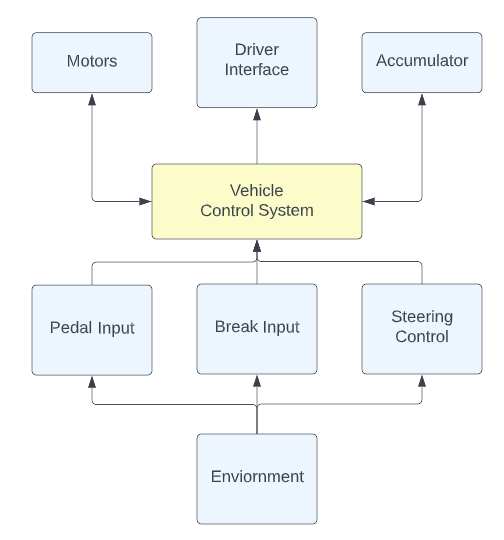
\includegraphics[width=10cm]{context_diagram.png}
    \caption{Control System Context Diagram}
    \label{fig:context_diagram}
\end{figure}

\begin{figure}[htp]
    \centering
    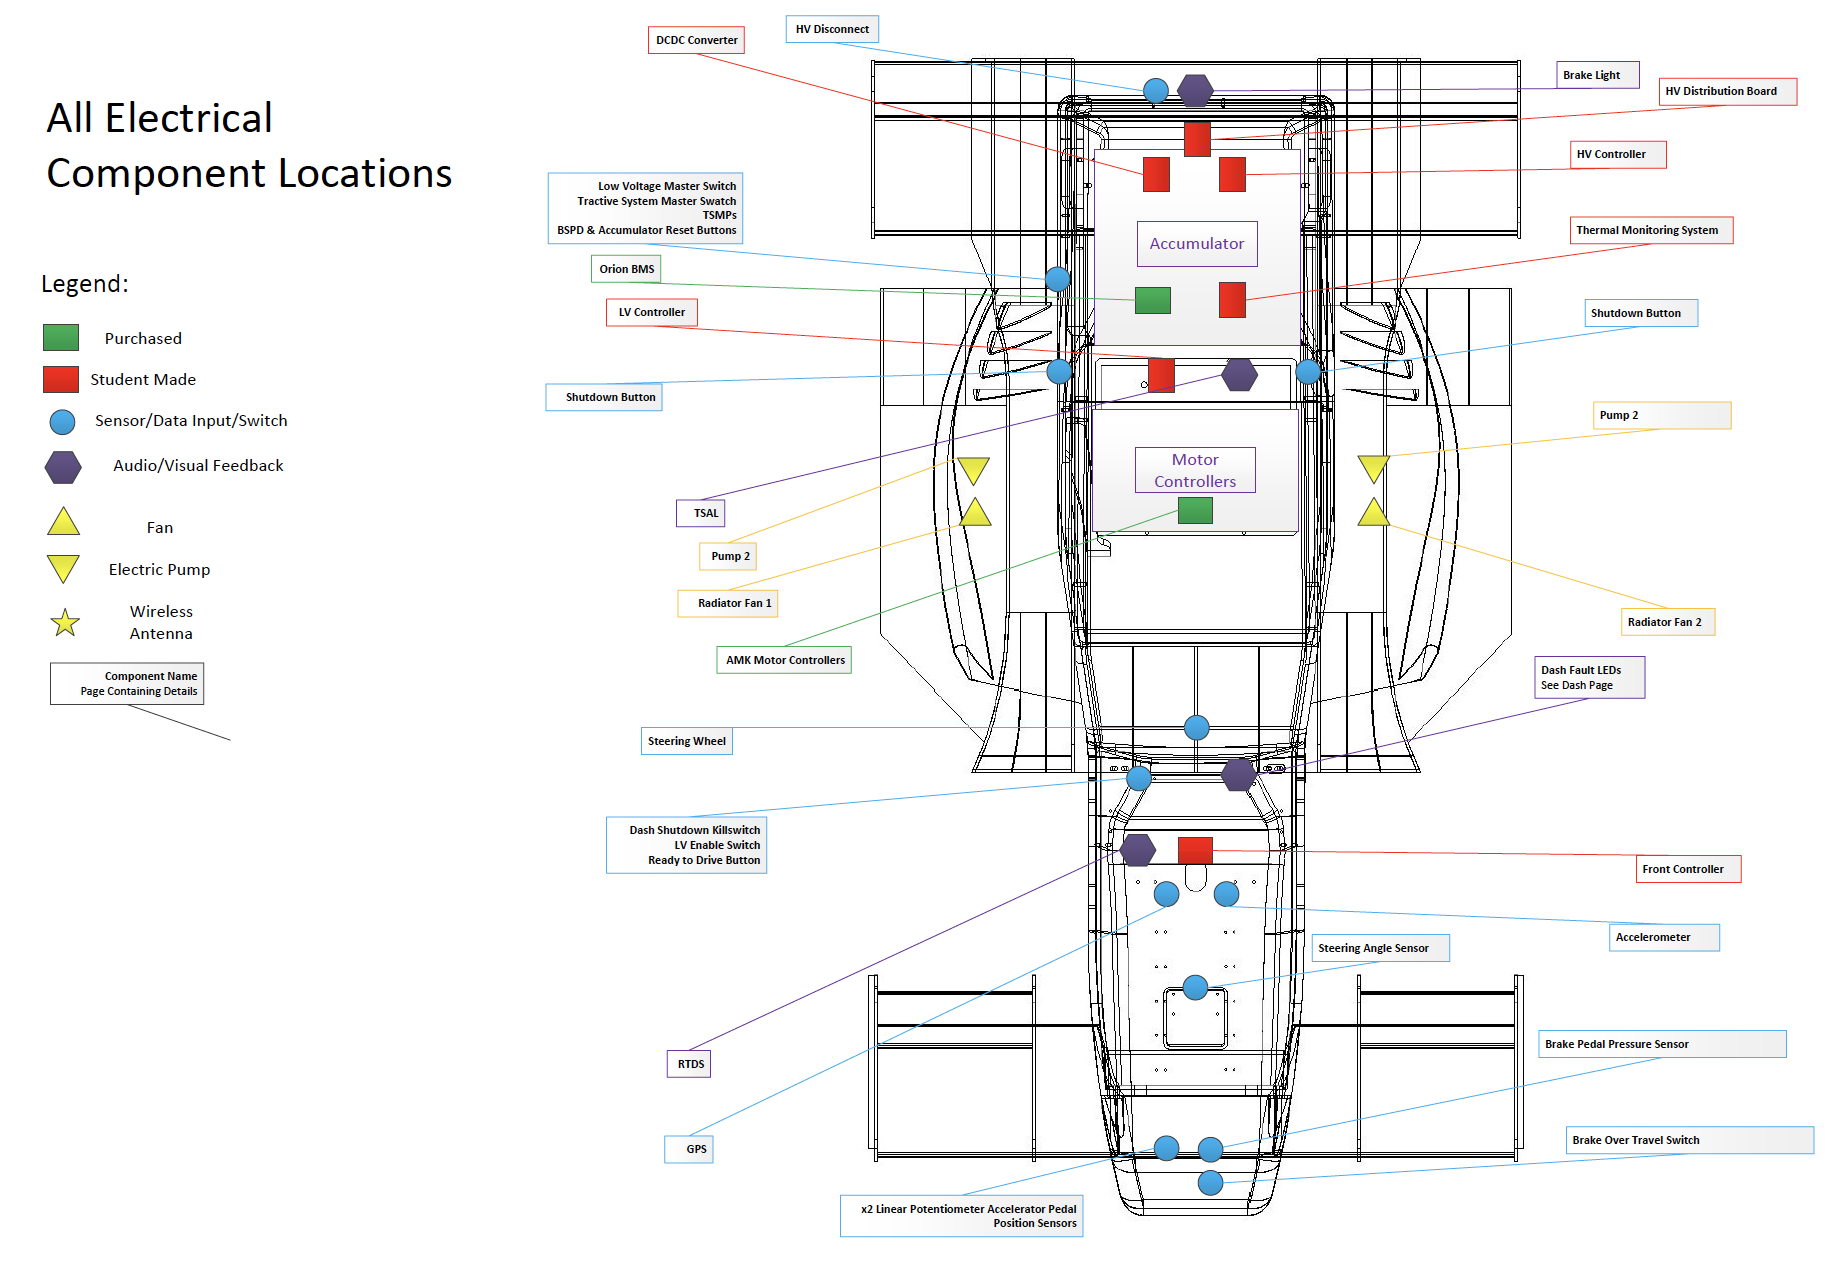
\includegraphics[width=15cm]{electrical_components.png}
    \caption{Electrical Component Context Diagram}
    \label{fig:electrical_component}
\end{figure}

\newpage
\section{Functional Decomposition Diagrams}

The following diagrams show monitor (input) and control (output) variables for each of the control system's subsystems. "Ring" is a common automotive industry term for model-based control program. As such, the MFE team refers to their vehicle control subsystems as Rings.\\

\noindent
\begin{figure}[htp]
    \centering
    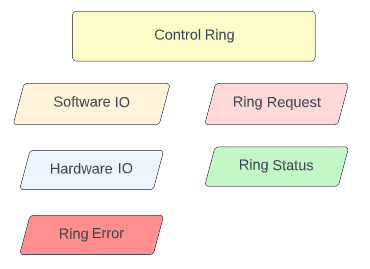
\includegraphics[width=8cm]{uml_legend.png}
    \caption{UML Color Coding Legend}
    \label{fig:uml_legend}
\end{figure}

\begin{figure}[htp]
    \centering
    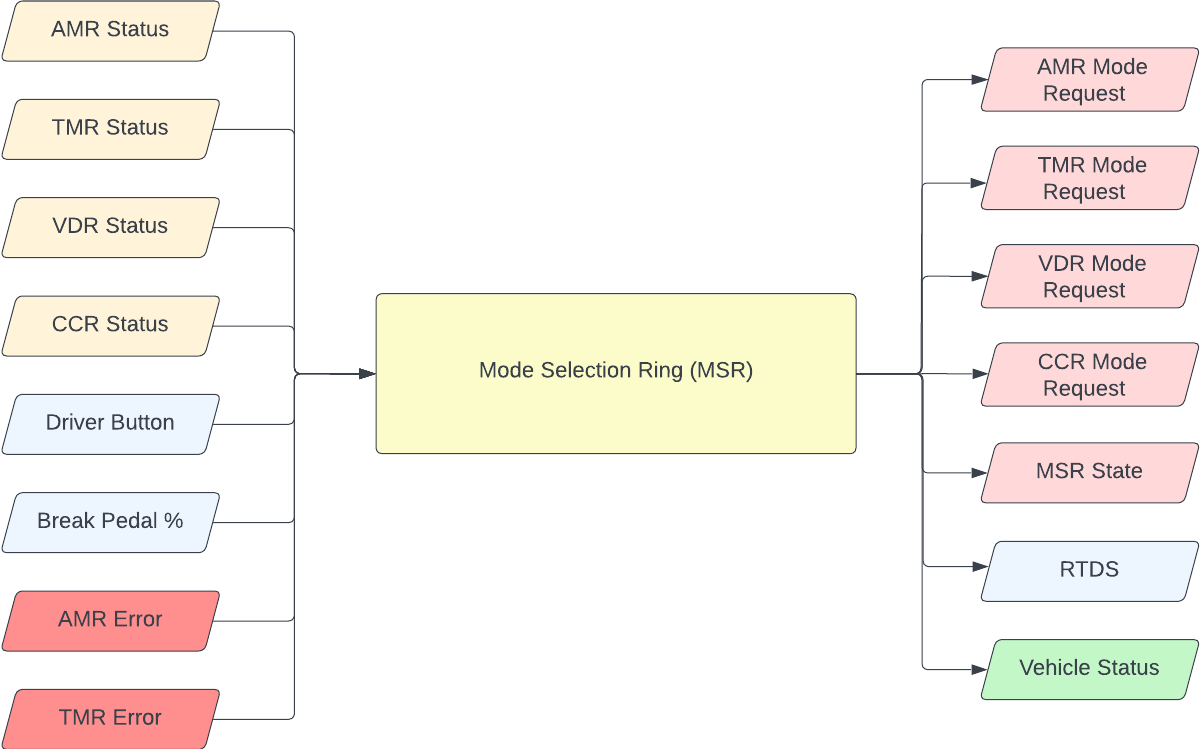
\includegraphics[width=15cm]{msr_uml.png}
    \caption{Mode Selection Ring UML}
    \label{fig:msr_uml}
\end{figure}

\begin{figure}[htp]
    \centering
    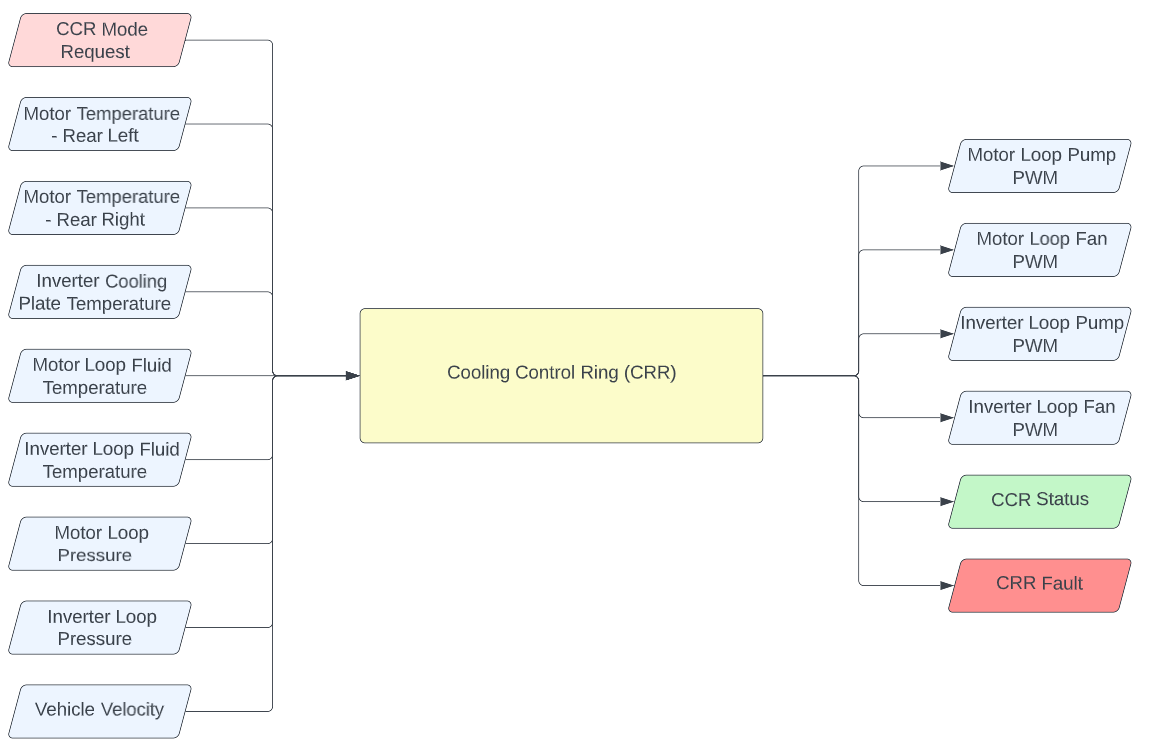
\includegraphics[width=15cm]{crr_uml.png}
    \caption{Cooling Control Ring UML}
    \label{fig:ccr_uml}
\end{figure}

\begin{figure}[htp]
    \centering
    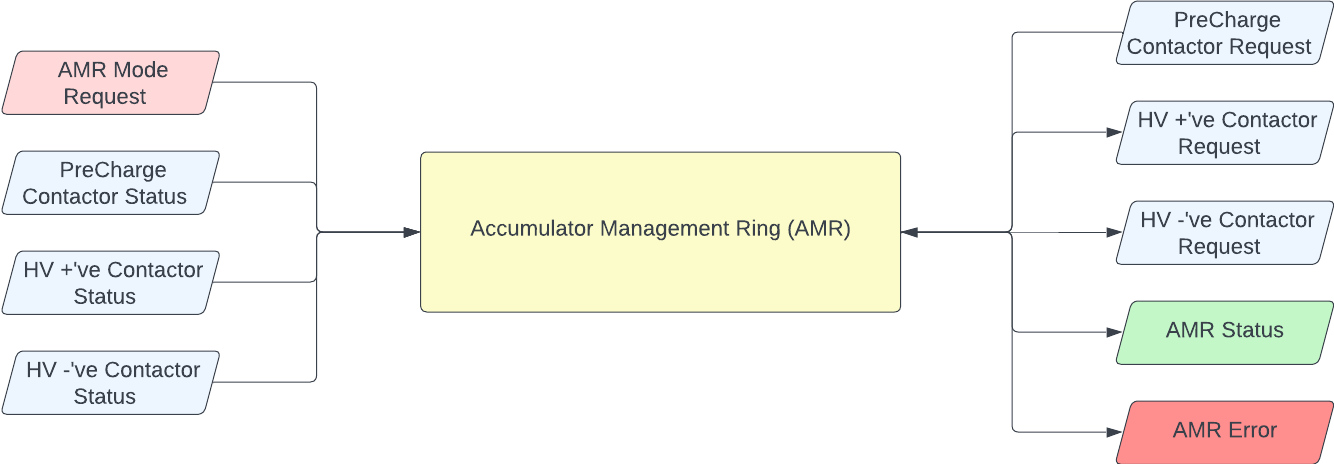
\includegraphics[width=15cm]{amr_uml.png}
    \caption{Accumulator Management Ring UML}
    \label{fig:amr_uml}
\end{figure}

\begin{figure}[htp]
    \centering
    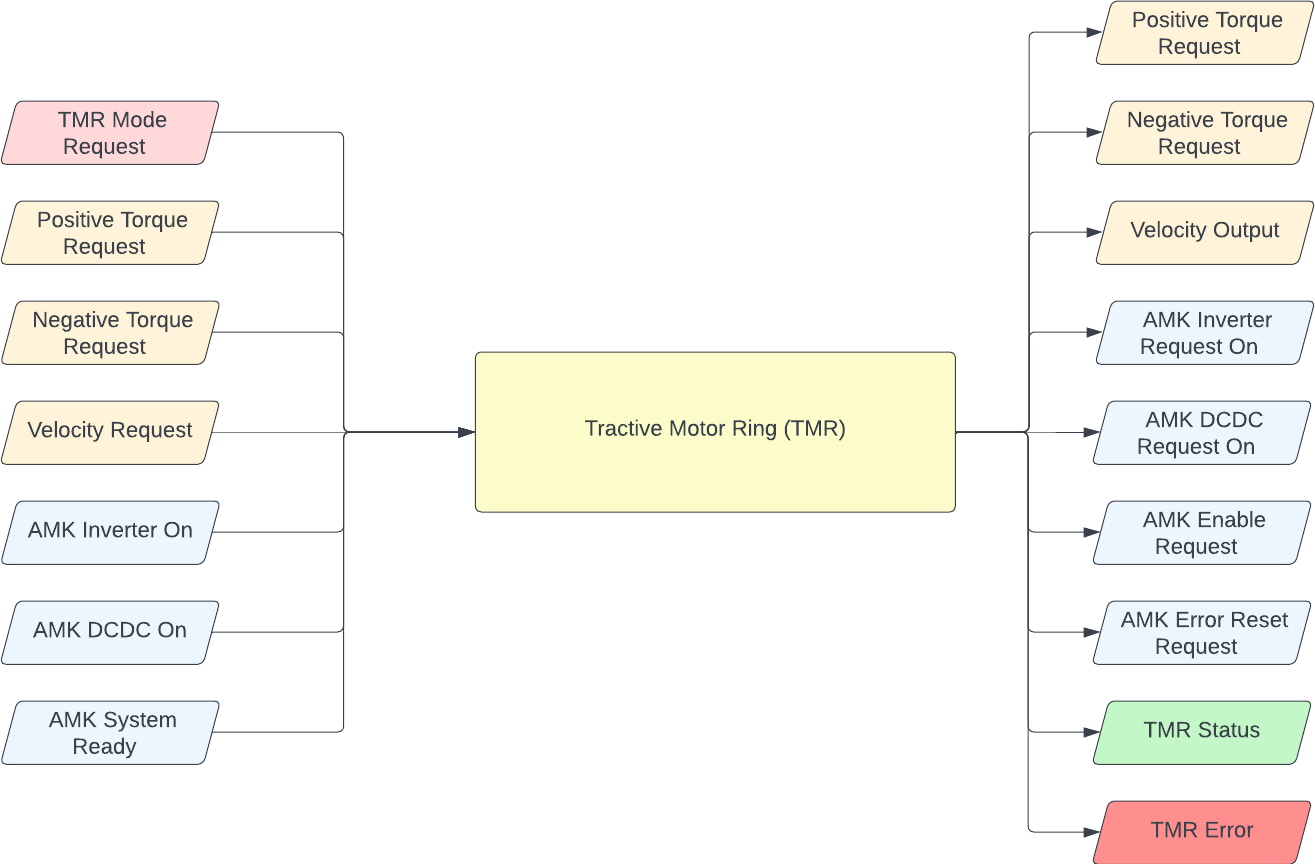
\includegraphics[width=15cm]{tmr_uml.png}
    \caption{Tractive Motor Ring UML}
    \label{fig:tmr_uml}
\end{figure}

\begin{figure}[htp]
    \centering
    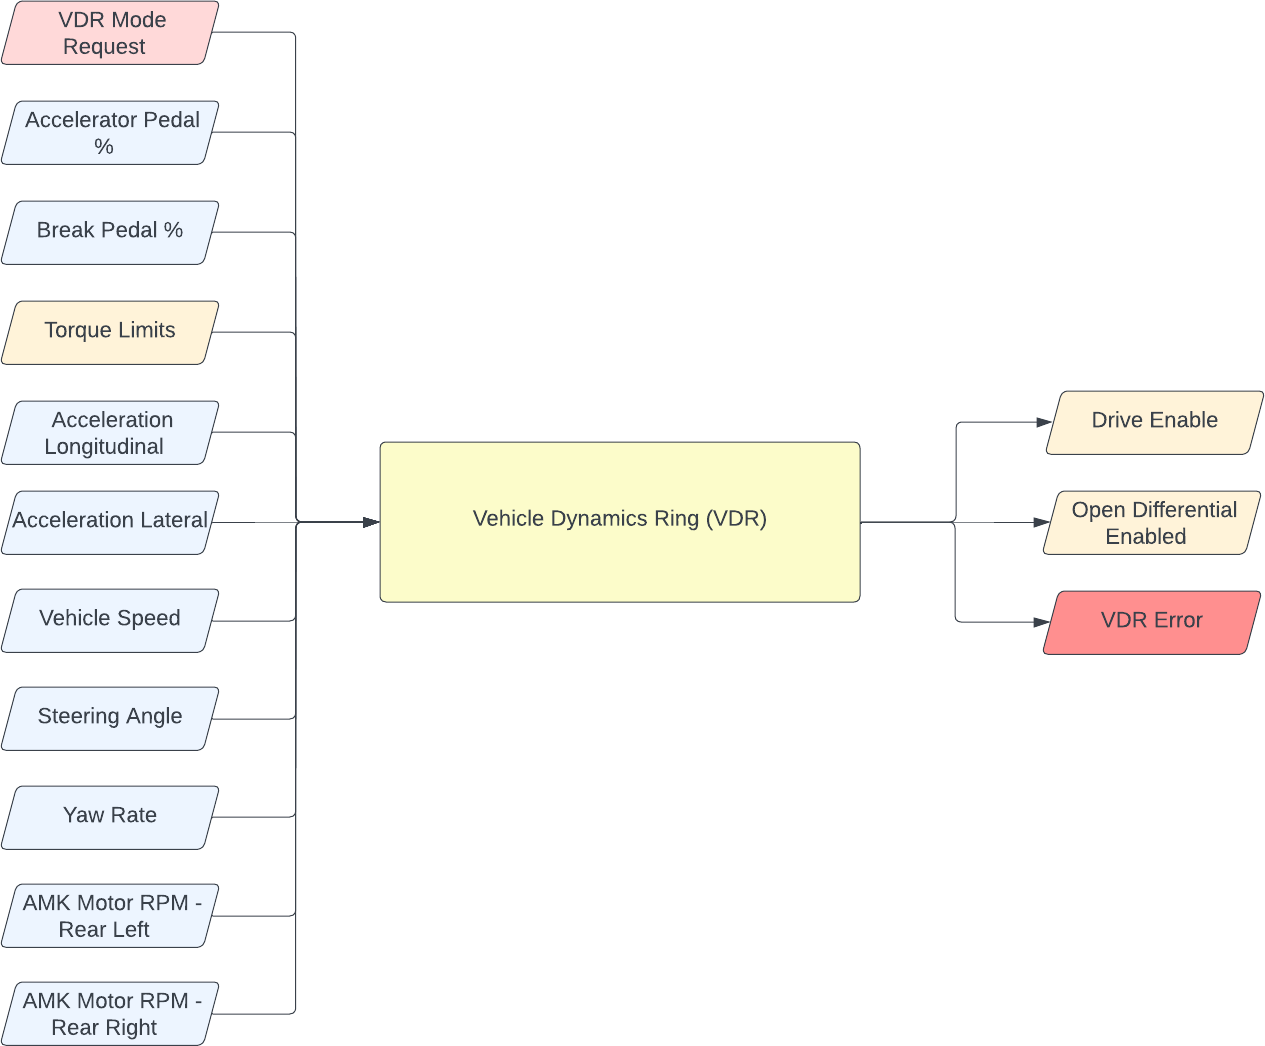
\includegraphics[width=15cm]{vdr_uml.png}
    \caption{Vehicle Dynamics Ring UML}
    \label{fig:vdr_uml}
\end{figure}

\newpage
\section{Functional Requirements}

\subsection{Accumulator Management Ring}


\begin{tabular}{| p{\ReqColA} | p{\ReqColB}|}
\hline
\rowcolor[gray]{0.9}
AMR1 & Accumulator Management control shall monitor the following inputs: AMR Mode Request, PreCharge Contactor Status, HV Positive Contactor Status, HV Negative Contactor Status.\\
\hline
Rationale & These inputs determine the state and control domain of the battery. \\
\hline
Likelihood of Change & Likely - More inputs may be needed as module complexity
grows. \\
\hline
\end{tabular}

\vspace{\tableVspace}
\noindent
\begin{tabular}{| p{\ReqColA} | p{\ReqColB}|}
\hline
\rowcolor[gray]{0.9}
AMR2 & Accumulator Management control shall compute the following output parameters: PreCharge Contactor Request, HV Positive Contactor Request, HV Negative Contactor Request, AMR Status, AMR Error.\\
\hline
Rationale &  Essential command signals and state reporting to other control system modules.\\
\hline
Likelihood of Change & Likely - More outputs may be needed as module complexity
grows. \\
\hline
\end{tabular}

\vspace{\tableVspace}
\noindent
\begin{tabular}{| p{\ReqColA} | p{\ReqColB}|}
\hline
\rowcolor[gray]{0.9}
AMR3 & Accumulator Management control shall not issue a contactor-close command during any fuse condition.\\
\hline
Rationale & Fusing refers to a contactor "welding" shut due to an electrical current spike, and can occur during high-load conditions.\\
\hline
Likelihood of Change & Very unlikely - Key functionality\\
\hline
\end{tabular}

\vspace{\tableVspace}
\noindent
\begin{tabular}{| p{\ReqColA} | p{\ReqColB}|}
\hline
\rowcolor[gray]{0.9}
AMR4 & Accumulator Management control shall adhere to FSAE EV.4.1.1 - "The maximum power drawn from the Accumulator [battery] must not exceed 80 kW."\\
\hline
Rationale & Competition rule \\
\hline
Likelihood of Change & Very unlikely - Competition rule \\
\hline
\end{tabular}

\vspace{\tableVspace}
\noindent
\begin{tabular}{| p{\ReqColA} | p{\ReqColB}|}
\hline
\rowcolor[gray]{0.9}
AMR5 & Accumulator Management control shall adhere to FSAE EV.4.1.2 - "The maximum permitted voltage that may occur between any two points must not exceed 600 V DC"\\
\hline
Rationale & Competition rule \\
\hline
Likelihood of Change & Very unlikely - Competition rule \\
\hline
\end{tabular}

\vspace{\tableVspace}
\noindent
\begin{tabular}{| p{\ReqColA} | p{\ReqColB}|}
\hline
\rowcolor[gray]{0.9}
AMR6 & Accumulator Management control shall adhere to FSAE EV.4.1.3 - "The powertrain must not regenerate energy when vehicle speed is between 0 and 5 km/hr"\\
\hline
Rationale & Competition rule \\
\hline
Likelihood of Change & Very unlikely - Competition rule \\
\hline
\end{tabular}

\vspace{\tableVspace}
\noindent
\begin{tabular}{| p{\ReqColA} | p{\ReqColB}|}
\hline
\rowcolor[gray]{0.9}
AMR7 & Accumulator Management control shall adhere to FSAE EV.4.2.1 - "Supplying power to the motor to drive the vehicle in reverse is prohibited"\\
\hline
Rationale & Competition rule \\
\hline
Likelihood of Change & Very unlikely - Competition rule \\
\hline
\end{tabular}

\vspace{\tableVspace}
\noindent
\begin{tabular}{| p{\ReqColA} | p{\ReqColB}|}
\hline
\rowcolor[gray]{0.9}
AMR8 & Accumulator Management control shall adhere to FSAE EV.4.2.1 - "Supplying power to the motor to drive the vehicle in reverse is prohibited"\\
\hline
Rationale & Competition rule \\
\hline
Likelihood of Change & Very unlikely - Competition rule \\
\hline
\end{tabular}

\vspace{\tableVspace}
\noindent
\begin{tabular}{| p{\ReqColA} | p{\ReqColB}|}
\hline
\rowcolor[gray]{0.9}
AMR9 & Accumulator Management control shall issue any other BMS commands in accordance with procedures outlined in the Orion BMS documentation.\\
\hline
Rationale & To ensure correct operation of the BMS kit.\\
\hline
Likelihood of Change & Very unlikely - Key functionality \\
\hline
\end{tabular}


\subsection{Cooling Control Ring}


\begin{tabular}{| p{\ReqColA} | p{\ReqColB}|}
\hline
\rowcolor[gray]{0.9}
CCR1 & Cooling Control shall monitor the following inputs: CCR Mode Request, Motor Temp Rear Left, Motor Temp Rear Right, Inverter Cooling Plate Temp, Motor Loop Fluid Temp, Inverter Loop Fliud Temp, Motor Loop Pressure, Inverter Loop Pressure, Vehicle Velocity.\\
\hline
Rationale & These aspects of the vehicle \& battery state must be known in order to send suitable commands to the cooling system. \\
\hline
Likelihood of Change & Likely - More inputs may be needed as module complexity
grows. \\
\hline
\end{tabular}

\vspace{\tableVspace}
\noindent
\begin{tabular}{| p{\ReqColA} | p{\ReqColB}|}
\hline
\rowcolor[gray]{0.9}
CCR2 & Cooling Control shall compute the following output parameters: Motor Loop Pump PWM, Motor Loop Fan PWM, Inverter Loop Pump PWM, Inverter Loop PWM, CCR Status, CCR Fault."\\
\hline
Rationale &  Essential command signals and state reporting to other control system modules.\\
\hline
Likelihood of Change & Likely - More outputs may be needed as module complexity
grows. \\
\hline
\end{tabular}

\vspace{\tableVspace}
\noindent
\begin{tabular}{| p{\ReqColA} | p{\ReqColB}|}
\hline
\rowcolor[gray]{0.9}
CCR3 & Cooling Control shall compute duty factors for each cooling loop such that temperatures remain within tractive system operation range.\\
\hline
Rationale &  Hardware operation limits\\
\hline
Likelihood of Change & Very unlikely - Hardware operation limit\\
\hline
\end{tabular}

\subsection{Mode Selection Ring}


\begin{tabular}{| p{\ReqColA} | p{\ReqColB}|}
\hline
\rowcolor[gray]{0.9}
MSR1 & Mode Selection shall monitor the following inputs: AMR Status, TMR Status, VDR Status, CCR Status, Driver Button, Brake Pedal \%, AMR Error, TMR Error\\
\hline
Rationale & These aspects of the vehicle state must be known in order to send suitable commands to the rest of the control system. \\
\hline
Likelihood of Change & Likely - More inputs may be needed as module complexity
grows. \\
\hline
\end{tabular}

\vspace{\tableVspace}
\noindent
\begin{tabular}{| p{\ReqColA} | p{\ReqColB}|}
\hline
\rowcolor[gray]{0.9}
MSR2 & Mode Selection shall compute the following output parameters: AMR Mode Request, TMR Mode Request, VDR Mode Request, CCR Mode Request, MSR State, RTDS, Vehicle Status"\\
\hline
Rationale &  Essential command signals and state reporting to other control system modules.\\
\hline
Likelihood of Change & Likely - More outputs may be needed as module complexity
grows. \\
\hline
\end{tabular}

\vspace{\tableVspace}
\noindent
\begin{tabular}{| p{\ReqColA} | p{\ReqColB}|}
\hline
\rowcolor[gray]{0.9}
MSR3 & Mode Selection shall adhere to Activation Sequence rule FSAE EV.10.4.1 ["Low Voltage (GLV) System"] - The Shutdown Circuit may be Closed when or after the GLV System is energized \\
\hline
Rationale & Competition rule\\
\hline
Likelihood of Change & Very unlikely - Competition rule \\
\hline
\end{tabular} 

\vspace{\tableVspace}
\noindent
\begin{tabular}{| p{\ReqColA} | p{\ReqColB}|}
\hline
\rowcolor[gray]{0.9}
MSR4 & Mode Selection shall adhere to Activation Sequence rule FSAE EV.10.4.2 ["Traction System Active"] 
\begin{itemize}
    \item Definition – High Voltage is present outside of the Accumulator Container
    \item Tractive System Active must not be possible until both: (1) GLV System is Energized; (2) Shutdown Circuit is Closed
\end{itemize} \\
\hline
Rationale & Competition rule\\
\hline
Likelihood of Change & Very unlikely - Competition rule \\
\hline
\end{tabular} 

\vspace{\tableVspace}
\noindent
\begin{tabular}{| p{\ReqColA} | p{\ReqColB}|}
\hline
\rowcolor[gray]{0.9}
MSR5 & Mode Selection shall adhere to Activation Sequence rule FSAE EV.10.4.3 ["Ready to Drive"] 
\begin{itemize}
    \item Definition – the Motor(s) will respond to the input of the APPS
    \item Ready to Drive must not be possible until: (1) Tractive System Active; (2) The brake pedal is pressed and held to engage the mechanical brakes; (3) The driver performs a manual action to initiate Ready to Drive
    such as pressing a specific button in the cockpit
\end{itemize} \\
\hline
Rationale & Competition rule\\
\hline
Likelihood of Change & Very unlikely - Competition rule \\
\hline
\end{tabular} 

\vspace{\tableVspace}
\noindent
\begin{tabular}{| p{\ReqColA} | p{\ReqColB}|}
\hline
\rowcolor[gray]{0.9}
MSR6 & Mode Selection shall adhere to Shutdown Circuit Operation rule FSAE EV.8.2.1 - The Shutdown Circuit must Open when any of the following exist:
\begin{itemize}
    \item Operation of, or detection from any of the components listed in EV.8.1.1
    \item Any shutdown of the GLV System
\end{itemize} \\
\hline
Rationale & Competition rule\\
\hline
Likelihood of Change & Very unlikely - Competition rule \\
\hline
\end{tabular} 

\vspace{\tableVspace}
\noindent
\begin{tabular}{| p{\ReqColA} | p{\ReqColB}|}
\hline
\rowcolor[gray]{0.9}
MSR7 & Mode Selection shall adhere to Shutdown Circuit Operation rule FSAE EV.8.2.2 - When the Shutdown Circuit Opens:
\begin{itemize}
    \item The Tractive System must Shutdown
    \item All Accumulator current flow must stop immediately
    \item The voltage in the Tractive System must be Low Voltage T.9.1.2 in five seconds or less
    \item The Motor(s) must spin free. Torque must not be applied to the Motor(s)
\end{itemize} \\
\hline
Rationale & Competition rule\\
\hline
Likelihood of Change & Very unlikely - Competition rule \\
\hline
\end{tabular} 

\vspace{\tableVspace}
\noindent
\begin{tabular}{| p{\ReqColA} | p{\ReqColB}|}
\hline
\rowcolor[gray]{0.9}
MSR8 & Mode Selection shall adhere to Shutdown Circuit Operation rule FSAE EV.8.2.3 - When the AMS, IMD or BSPD Open the Shutdown Circuit:
\begin{itemize}
    \item The Tractive System must remain disabled until manually reset 
    \item The driver must not be able to reactivate the Tractive System from inside the vehicle
    \item Operation of the Shutdown Buttons or TSMS must not reset the Shutdown Circuit
    \item The Tractive System must be reset only by manual action of a person directly at the vehicle
\end{itemize} \\
\hline
Rationale & Competition rule\\
\hline
Likelihood of Change & Very unlikely - Competition rule \\
\hline
\end{tabular} 

\vspace{\tableVspace}
\noindent
\begin{tabular}{| p{\ReqColA} | p{\ReqColB}|}
\hline
\rowcolor[gray]{0.9}
VSM9 & Mode Selection shall adhere to Shutdown Circuit Operation rule FSAE EV.8.2.4 - The driver may reset the Shutdown Circuit from the cockpit, subject to EV.8.2.3 \\
\hline
Rationale & Competition rule\\
\hline
Likelihood of Change & Very unlikely - Competition rule \\
\hline
\end{tabular} 

\subsection{Tractive Motor Ring}

\begin{tabular}{| p{\ReqColA} | p{\ReqColB}|}
\hline
\rowcolor[gray]{0.9}
TMR1 & Tractive Motor control shall monitor feedback signals from
the AMK motor controller: AMK Inverter On, AMK DCDC On, AMK System Ready.\\
\hline
Rationale & The current motor state must be known in order to send suitable
commands to the motor controller.\\
\hline
Likelihood of Change & Very unlikely - Key functionality \\
\hline
\end{tabular} \\

\vspace{\tableVspace}
\noindent
\begin{tabular}{| p{\ReqColA} | p{\ReqColB}|}
\hline
\rowcolor[gray]{0.9}
TMR2 & Tractive Motor control shall also monitor the following inputs: TMR Mode Request, Positive Torque Request, Negative Torque Request, Velocity Request.\\
\hline
Rationale & Certain aspects of the vehicle state must be known in order to send suitable commands to the motor controller.\\
\hline
Likelihood of Change & Very unlikely - Key functionality \\
\hline
\end{tabular} \\

\vspace{\tableVspace}
\noindent
\begin{tabular}{| p{\ReqColA} | p{\ReqColB}|}
\hline
\rowcolor[gray]{0.9}
TMR3 & Tractive Motor control shall issue motor commands in accordance
with procedures outlined in the AMK documentation.\\
\hline
Rationale & To ensure correct operation of the motor kit.\\
\hline
Likelihood of Change & Very unlikely - Key functionality \\
\hline
\end{tabular} \\

\vspace{\tableVspace}
\noindent
\begin{tabular}{| p{\ReqColA} | p{\ReqColB}|}
\hline
\rowcolor[gray]{0.9}
TMR4 & Tractive Motor control shall compute the following output parameters: Positive Torque Request, Negative Torque Request, Velocity Output, AMK Inverter Request On, AMK DCDC Request On, AMK Enable Request, AMK Error Reset Request, TMR Status, TMR Error."\\
\hline
Rationale &  Essential command signals and state reporting to other control system modules.\\
\hline
Likelihood of Change & Likely - More outputs may be needed as module complexity
grows. \\
\hline
\end{tabular}

\vspace{\tableVspace}
\noindent
\begin{tabular}{| p{\ReqColA} | p{\ReqColB}|}
\hline
\rowcolor[gray]{0.9}
TMR5 & Tractive Motor control shall adhere to FSAE EV.4.2.3 - "Any algorithm or electronic control unit that can adjust the requested wheel torque may only
lower the total driver requested torque and must not increase it"\\
\hline
Rationale & Competition rule\\
\hline
Likelihood of Change & Very unlikely - Competition rule \\
\hline
\end{tabular} \\

\vspace{\tableVspace}
\noindent
\begin{tabular}{| p{\ReqColA} | p{\ReqColB}|}
\hline
\rowcolor[gray]{0.9}
TMR6 & Tractive Motor control shall adhere to FSAE EV.5.7.1 - "The power to the Motor(s) must be immediately and completely shut down when the two of these exist at the same time: (1) The mechanical brakes are engaged; (2) The APPS signals more than 25\% pedal travel"\\
\hline
Rationale & Competition rule \\
\hline
Likelihood of Change & Very unlikely - Competition rule \\
\hline
\end{tabular}

\vspace{\tableVspace}
\noindent
\begin{tabular}{| p{\ReqColA} | p{\ReqColB}|}
\hline
\rowcolor[gray]{0.9}
TMR7 & Tractive Motor control shall adhere to FSAE EV.5.7.2 - "The Motor shut down must remain active until the APPS signals less than 5\% pedal travel, with
or without brake operation."\\
\hline
Rationale & Competition rule \\
\hline
Likelihood of Change & Very unlikely - Competition rule \\
\hline
\end{tabular}

\subsection{Vehicle Dynamics Ring}


\begin{tabular}{| p{\ReqColA} | p{\ReqColB}|}
\hline
\rowcolor[gray]{0.9}
VDR1 & Vehicle Dynamics control shall monitor the following inputs: VDR Mode Request, Accelerator Pedal \%, Brake Pedal \%, Torque Limits, Longitudinal Acceleration, Lateral Acceleration, Vehicle Speed, Steering Angle, Yaw Rate, AMK Motor RPM Rear Left/Right\\
\hline
Rationale & These aspects of the vehicle state must be known in order to send suitable commands to the rest of the control system. \\
\hline
Likelihood of Change & Likely - More inputs may be needed as module complexity
grows. \\
\hline
\end{tabular}

\vspace{\tableVspace}
\noindent
\begin{tabular}{| p{\ReqColA} | p{\ReqColB}|}
\hline
\rowcolor[gray]{0.9}
VDR2 & Vehicle Dynamics control shall compute the following output parameters: Drive Enable, Open Differential Enable, VDR Error"\\
\hline
Rationale &  Essential command signals and state reporting to other control system modules.\\
\hline
Likelihood of Change & Likely - More outputs may be needed as module complexity
grows. \\
\hline
\end{tabular}

% \section{Functional Requirements Likelihood of Change}

% \subsection{Accumulator Management}
% \subsection{Cooling Control}
% \subsection{Mode Selection}
% \subsection{Tractive Motor}
% \subsection{Vehicle Dynamics}

\section{Non-Functional Requirements}

\subsection{Look and Feel Requirements}
The control system has no "front-end" that would drive user-facing look and feel requirements. 

\vspace{\tableVspace}
\noindent
\begin{tabular}{| p{\ReqColA} | p{\ReqColB}|}
\hline
\rowcolor[gray]{0.9}
NFR1 & The control system Simulink models shall follow a standardized
format that facilitates readability and encapsulation.\\
\hline
Rationale &  Future FSAE students should be able to understand control logic while consulting as little documentation as possible. \\
\hline
\end{tabular}

\subsection{Usability Requirements}
The control system will not be directly interacted with by a user. 

\vspace{\tableVspace}
\noindent
\begin{tabular}{| p{\ReqColA} | p{\ReqColB}|}
\hline
\rowcolor[gray]{0.9}
NFR2 & The control system build target shall be the team-selected microcontroller platform, STM32F7\\
\hline
Rationale &  Software compatibility with the end-use hardware.\\
\hline
\end{tabular}

\subsection{Performance Requirements}
\begin{tabular}{| p{\ReqColA} | p{\ReqColB}|}
\hline
\rowcolor[gray]{0.9}
NFR3 & Running the control system on the embedded controller shall not exceed the computational throughput of the controller.  \\
\hline
Rationale & To ensure vehicle safety expectations and competition rules are met, and to ensure vehicle performance is as desired.\\
\hline
\end{tabular}

\subsection{Maintainability and Support Requirements}

\begin{tabular}{| p{\ReqColA} | p{\ReqColB}|}
\hline
\rowcolor[gray]{0.9}
NFR4 & The control system shall make use of hardware abstraction modules, that have consistent outputs to our system regardless of changing the underlying hardware.\\
\hline
Rationale & Future hardware changes can be accommodated within their own encapsulated modules rather than requiring control logic models. \\
\hline
\end{tabular}

\vspace{\tableVspace}\noindent
\begin{tabular}{| p{\ReqColA} | p{\ReqColB}|}
\hline
\rowcolor[gray]{0.9}
NFR5 & The control system modules shall incorporate modularization principles, including encapsulation and information hiding.\\
\hline
Rationale & Having modules and sub-modules interact through well-defined inputs/outputs, while hiding their implementation, facilitates maintainability by allowing module implementation updates to not drive downstream changes.  \\
\hline
\end{tabular}

\vspace{\tableVspace}\noindent
\begin{tabular}{| p{\ReqColA} | p{\ReqColB}|}
\hline
\rowcolor[gray]{0.9}
NFR6 & The control system modules shall be documented according to a standardized, team-approved format.\\
\hline
Rationale & Facilitate effective knowledge transfer to future FSAE students. \\
\hline
\end{tabular}

\subsection{Security Requirements}

Code-level security is not within the scope of the project. However, access to source code and high-level control logic is. \\

\vspace{\tableVspace}\noindent
\begin{tabular}{| p{\ReqColA} | p{\ReqColB}|}
\hline
\rowcolor[gray]{0.9}
NFR7 & The control system repository shall be public for the duration of the capstone project. \\
\hline
Rationale & Open visiblity for marking and accountability. \\
\hline
\end{tabular}

\vspace{\tableVspace}\noindent
\begin{tabular}{| p{\ReqColA} | p{\ReqColB}|}
\hline
\rowcolor[gray]{0.9}
NFR8 & The control system repository shall be made private upon completion of the project.\\
\hline
Rationale & To prevent our team's work being copied by a rival team, as this can cause issues in terms of plagiarism as per the FSAE rules, while also in practise reducing our competitive advantage.\\
\hline
\end{tabular}

\subsection{Cultural and Political Requirements}
As this is a competition-only vehicle with strict guidelines from SAE, there are no
relevant requirements reflecting on societal politics and culture.

\subsection{Legal Requirements}
As this is a competition-only vehicle with strict guidelines from SAE, there are no relevant legal requirements from governing bodies (that would not already been implicitly required with the SAE guidelines). 

\subsection{Health and Safety Requirements}

\vspace{\tableVspace}\noindent
\begin{tabular}{| p{\ReqColA} | p{\ReqColB}|}
\hline
\rowcolor[gray]{0.9}
NFR9 & The control system shall follow FSAE guidelines for safe energizing sequences. \\
\hline
Rationale & Most electric-related vehicle safety features (eg. emergency stops, fuses) are handled on the hardware level.\\
\hline
\end{tabular}

\vspace{\tableVspace}\noindent
\begin{tabular}{| p{\ReqColA} | p{\ReqColB}|}
\hline
\rowcolor[gray]{0.9}
NFR10 & If the vehicle is in motion while an unsafe condition occurs, the control system shall zero the motor torque commands until a system reset.\\
\hline
Rationale & The vehicle's "safe state" should be to allow the driver to coast or brake to a safe location, without issuing any positive/negative torque command from the motors.\\
\hline
\end{tabular}

\section{Project Issues}

\subsection{Open Issues}
Issues that have been raised and do not yet have a conclusion.
\begin{itemize}
    \item Version control mechanism needs to be instantiated for Simulink model development.  
    \item Sourcing and/or development of plant models to use in Model-in-loop testing is an open issue.
\end{itemize}

\subsection{Off-the-Shelf Solutions}
As this competition follows strict requirements from FSAE, a unique control system must be developed by each team. Systems provided by Mathworks and/or hardware manufacturers cannot be used beyond acting as a broad inspiration or syntax reference. 
Purchasing vehicle control software from a automotive supplier (eg. Bosch) would still require customization in order to meet FSAE competition requirements. 

\subsection{Risks}
\begin{itemize}
    \item The FSAE vehicle may not be ready by end-of-project to do vehicle level integration. 
    \item The embedded hardware may not be ready by end-of-project to do hardware-level integration. 
    \item Hardware-level testing introduces some health and safety risk.
    \item The team-selected microcontroller (STM32F7) may not have computational capacity required for a functional control system.
\end{itemize}

\begin{itemize}
    \item Roadblocks caused by MFE that are out of the team's control
\end{itemize}

\subsection{Costs}
Listed below are the costs associated with any hardware required to help design our product.

\vspace{3mm}
\noindent
\begin{tabular}{| p{0.65\textwidth} | p{0.3\textwidth}|}
\hline
\rowcolor[gray]{0.9}
Item & Price \\
\hline
\href{https://www.digikey.ca/en/products/detail/stmicroelectronics/NUCLEO-F767ZI/6004740}{NUCLEO-F767ZI Debugger}& \$25 \\
\hline
\end{tabular}
\\

\subsection{Waiting Room}

The following are the additions to the project that would be tackled after initial release of the product.

\begin{enumerate}[(i)]
    \item Vehicle Stability Control Program
    \item Torque Vectoring
    \item Over-the-air Data Acquisition
\end{enumerate}

% \begin{itemize}
%     \item 
% \end{itemize}

\section*{Appendix --- Reflection}

This project requires a team-wide understanding of developing embedded software that is functionally complete, robust, maintainable and documented, as well as working within a continuous-improvement framework. Other mechatronics-specific knowledge 
includes model-based design, signal conditioning, V-model development, requirements-based testing, software-simulation and physical modelling environments and state machine design. Broader technical knowledge will be developed in electric vehicles 
and automotive standards. Team members will need to be adept with various industry tools including Git, MATLAB/Simulink and LaTeX. Transferable skills are numerous, but notably include experience in compliance-driven design, design communication and 
collaborative project management.\\
\vspace{3mm}\noindent
\begin{tabular}{| p{0.2\textwidth} | p{0.75\textwidth}|}
    \hline
    \rowcolor[gray]{0.9}
    Team Member & Knowledge/Skills to develop  \\
    \hline
    Dharak & Software simulation \& physical system modelling, project management, integration testing, software design documentation \\
    \hline
    Abhishek & Embedded software development, design communication, model-based design, V-model, control system theory \\
    \hline
    Jason & Embedded software development, design communication, Simulink algorithms, predictive and intelligent control, real time applications with controls\\
    \hline
    Laura & Embedded software development, design communication, Simulink, knowledge of electric vehicles and their subsystems \\
    \hline
    Derek & Embedded software development, design communication, signal conditioning, state machine design, LaTeX, Git \\
    \hline
\end{tabular}

\newpage
Approaches and rationale are as follows.\\

\vspace{5mm}
\noindent
\begin{tabular}{| p{0.2\textwidth} | p{0.75\textwidth}|}
    \hline
    \rowcolor[gray]{0.9}
    Team Member & Knowledge/Skills to develop  \\
    \hline
    Dharak & To acquire knowledge and master the aforementioned skills, I could begin by (1) documenting my work and experience I have gained over my 6 years on MFE in order to easily transfer it down to my team members, (2) consult the expansive 
    catalog of resources provided by decorated FSAE Teams online, and (3) take a leading role in managing both the technical and admin work of the capstone group. Of the listed methods, I will be pursuing method (1) to build my knowledge and skill 
    set. As I have prior experience with embedded software, vehicle controls, and project management due to my past and current involvement with MFE, the best way for me to be able to reinforce the skills I have gained and applied is to reflect back
     upon them by documenting and teaching others. I strongly believe the best way to test ones knowledge on a topic is by explaining it to someone else, so by explaining the topics related to my goals to my team members, I will be reinforcing my own 
     understanding and be able to find any holes in my own knowledge.\\
    \hline
    Abhishek & To enhance the skills I've listed above, I can (1) make use of great professors that are available to us, like Professor Lawford, that have a deep understanding of vehicle control systems (2) put into practice what I've learned in 
    multiple courses during my time at McMaster eg. Real Time Applications and Intelligent Control, and finally (3) make use of the great FSAE Formula Electric community to fill any gaps in understanding I may have. Having previous co-ops in the 
    controls space, I will be using what I've learned from practical experience and theoretical experience to become a great asset to this project's development and final outcome. \\
    \hline
    Jason & Build on course work I have done based around software development and control theory. Additionally, being able to actually develop a control algorithm for on a vehicle is a very unique opportunity and so being able to grasp skills in
     all areas of it is important to me. Working on simulink for the model driven design pacemaker project provided a great introduction into simulink and I want to build on this skill set through this project. Through conducting research on vehicle
      controls algorithms, or through consulting professors, I will aim to complete my goal. From the above approaches, I will be pursuing the approach of working with professors, such as Dr. Martin v. Mohrenschildt as he is an expert in the control 
      systems area.\\
    \hline
\end{tabular}
\begin{tabular}{| p{0.2\textwidth} | p{0.75\textwidth}|}
    \hline
    Laura & To ensure that I acquire the skills and knowledge listed above, I will thoroughly review the documentation provided by the MFE team. I will also do research on other electric vehicles, especially ones that are available commercially, to 
    keep up with the ongoing demands and trends of the industry. This will help me to make sure I am on track with my team and that I fully understand the scope of the project and can make meaning contributions to the team. As I have previous experience 
    with software development and design communication, I will be focusing on continuing to learn about electrical vehicles and their subsystems.\\
    \hline
    Derek & Though I have some experience in state-machine design, formal documentation in LaTeX, and in Git, these have been for smaller-scale projects where I could get by with just the basics. This project provides the opportunity to deepen by knowledge 
    by applying these skills to a larger (in module count) and more complex system. I can enhance these skills by (1) taking advantage of the talent-base of the FSAE team by consulting team members for their knowledge and design advice, and (2) taking 
    advantage of the support from the Capstone instruction team, by consulting with the instructors/TAs for their best-use practices.\\
    \hline
\end{tabular}

\end{document}

